%!TEX root = labo.tex

\chapter{Static Routing}

What you will learn in this lab:

\begin{itemize}
	\item How to turn a computer with multiple interfaces into a router
	\item How to set up static routing on Linux PC-routers and Cisco commercial routers
	\item How ICMP messages update routing table entries
	\item How Proxy ARP helps to connect different networks without reconfiguring the hosts
	\item How to work with different network prefixes
\end{itemize}

\newpage
\setsession{prelab3}
\section{Prelab 3}\label{sec:prelab3}
%!TEX root = labo.tex

\subsubsection*{Network Commands in Linux}
Read the manual pages of the following commands at \url{http://manpages.ubuntu.com/} for the operating system version ``\osversion'':
\begin{itemize}
	\item \cmd{route}
	\item \cmd{traceroute}
	\item \cmd{minicom}: This lab uses the \cmd{minicom} utility program to establish a serial connection between a Linux PC and a Cisco router.
\end{itemize}

\subsubsection*{{Proxy ARP}}
Go to the website of Cisco at \url{http://goo.gl/ixuktT} and read about Proxy ARP.

\subsubsection*{Cisco IOS}
The Cisco routers in the Lab are running a recent version of the Cisco Internet Operating System (IOS). Read about the IOS at \url{http://goo.gl/UD23vX}. Note that this is reference material that you can use. You are not expected to go through all of the manuals listed here!

\remark The most useful manuals for this course are the ``IP Application Services Configuration Guide'' and ``Cisco IOS IP Switching Configuration Guide''.

\newpage
\subsection*{Prelab Questions}

\begin{questions}
	\q{1}{What is the IOS command to change the MTU (maximum transmission unit) for an interface on a Cisco router?}
	\q{2}{How does a router determine whether a datagrams to particular host can be directly delivered through one of its interfaces?}
	\q{3}{Which systems generate ICMP Route Redirect messages? Routers, hosts, or both?}
	\q{4}{What is the default maximum TTL value used by traceroute when sending UDP datagrams?}
	\q{5}{Describe the role of a default gateway in a routing table?}
	\q{6}{What is the network prefix of IP address 192.110.50.3/24?}
	\q{7}{Explain the difference between an IP address and a network prefix.}
	\q{8}{An organization has been assigned the network number 140.25.0.0/16 and it needs to create networks that support up to 60 hosts on each IP network. What is the maximum number of networks that can be set up? Explain your answer.}
\end{questions}


\newpage
\setsession{lab3}
\section{Lab 3}\label{sec:lab3}

In this lab you work with four different network topologies. The topology for Parts 1-4 is shown in Figure \ref{fig:lab3-network1}. These parts address router configuration on a Linux PC and a Cisco Router. The topology for Part 5 is shown in Figure \ref{fig:lab3-network2}. This topology is used to study the role of ICMP route redirect message. For Part 6 we add one more router to the topology of Part 5 and examine the effect of routing loops as displayed in Figure \ref{fig:lab3-network3}. The topology for Part 7 is shown in Figure \ref{fig:lab3-network4}. There, you explore the relationship between network prefixes and IP forwarding.

%FIXME: subfigures in memoire...
%\begin{figure}
%	\centering
%	\subbottom[Part 1 - 4]{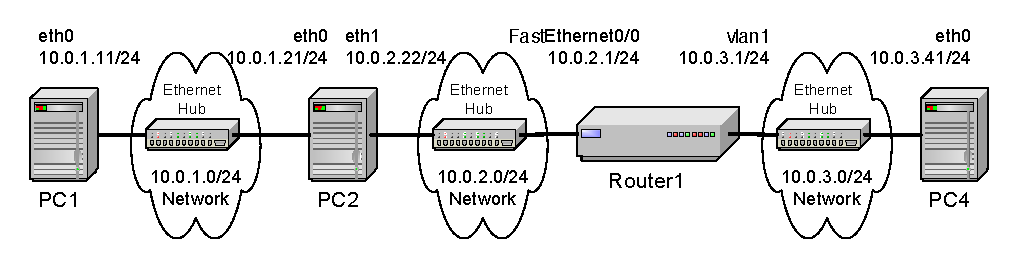
\includegraphics[width=0.4\linewidth]{graphics/lab3-network1-updated.pdf}}
%	\subbottom[Part 5]{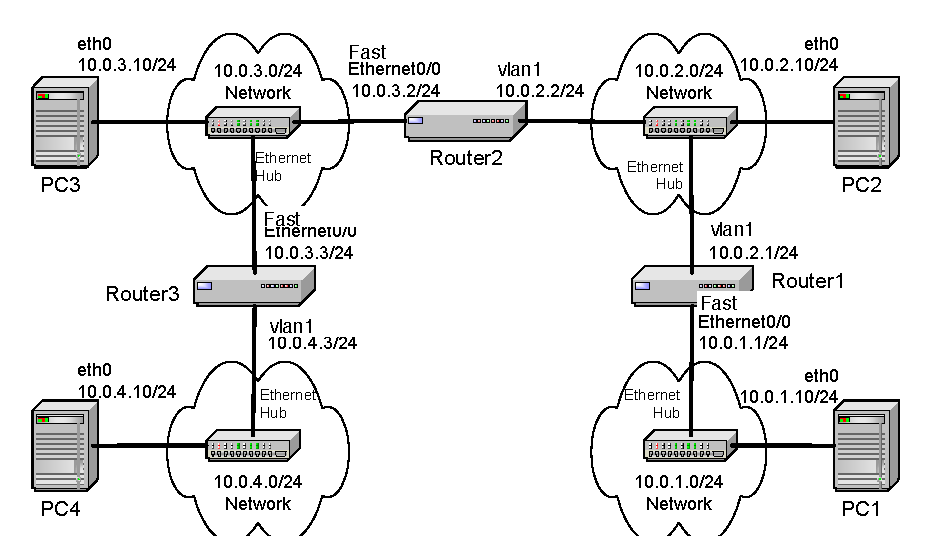
\includegraphics[width=0.4\linewidth]{graphics/lab3-network2-updated.pdf}}
%	\subbottom[Part 6]{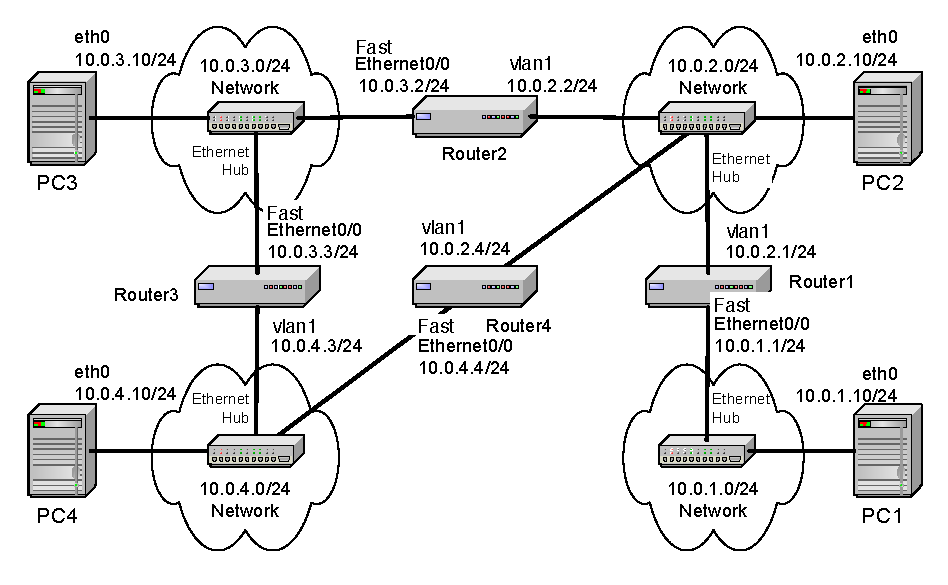
\includegraphics[width=0.4\linewidth]{graphics/lab3-network3-updated.pdf}}
%	\subbottom[Part 7]{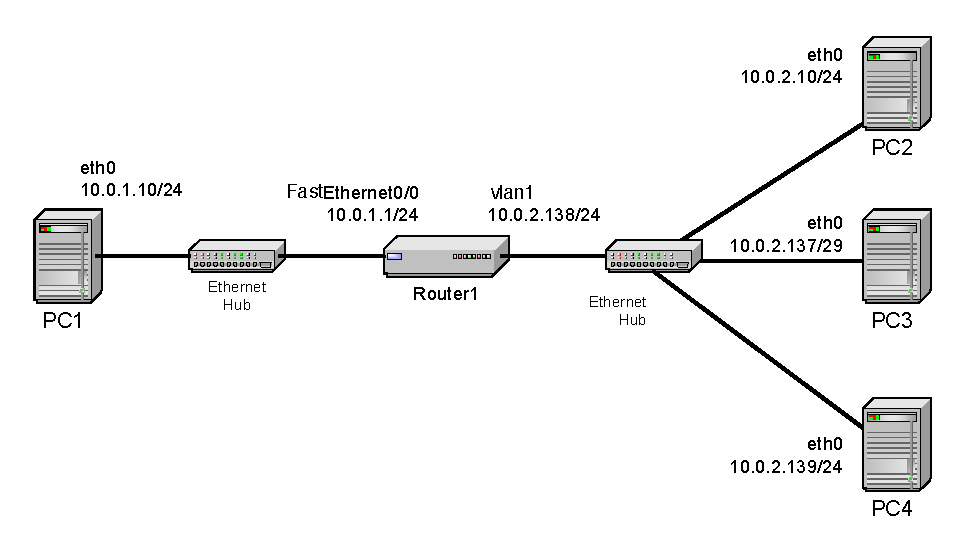
\includegraphics[width=0.4\linewidth]{graphics/lab3-network4-updated.pdf}}
%	\caption{Overview of the networks used in Lab \thechapter}
%  \label{fig:lab3-overview-networks}
%\end{figure}


\newpage
\subsection{Configuring a Linux PC as a Router}
Any Linux PC with at least two network interfaces can be set up as an IP router. Configuring a Linux PC as an IP router involves two steps: (1) modifying the configuration of Linux, so that IP forwarding is enabled and (2) configuring the routing table . Figure \ref{fig:lab3-network1} shows the network topology used in Parts 1 - 4 of this lab. PC1 and PC4 are used as hosts, and PC2 and Router1 are set up as IP routers. The PCs and the Cisco router are connected by three Ethernet hubs. In Lab 3, all routing table entries are manually configured, a procedure known as static routing.

\begin{figure}[h!t]
	\centering
	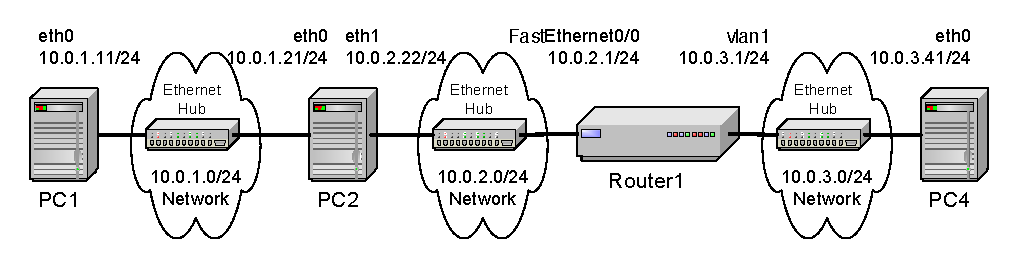
\includegraphics[width=\linewidth]{graphics/lab3-network1-updated.pdf}	
	\caption{Network configuration for Parts 1-4}
	\label{fig:lab3-network1}
\end{figure}

\begin{table}[h!t]
	\centering
	\begin{tabular}{| c | c | c |}	
		\hline
		\textbf{Linux PC} & \textbf{eth0} & \textbf{eth1} \\ \hline
		PC1 & 10.0.1.11/24 & Disabled \\ 
		PC2 & 10.0.1.21/24 & 10.0.2.22/24 \\
		PC3 & 10.0.3.41/24 & Disabled \\ \hline
		\textbf{Cisco Router} & \textbf{FastEthernet0/0} & \textbf{vlan1} \\ \hline
		Router1 & 10.0.2.1/24 & 10.0.3.1/24 \\ \hline
	\end{tabular}
	\caption{IP addresses for Parts 1-4}
	\label{tab:lab3-network1}
\end{table}

\subsubsection*{Exercise 1-A. Network setup}

\begin{enumerate}
	\item  Connect the Ethernet interfaces of the Linux PCs and the Cisco router as shown in Figure \ref{fig:lab3-network1}. Configure the IP addresses of the interfaces as given in Table \ref{tab:lab3-network1}.
	\item Start to capture traffic on PC1 with Wireshark.
	\item Issue a \cmd{ping} command from PC1 to PC2, Router1 and PC4. Save the output of each \cmd{ping} command.
		\begin{cmdblock}
PC1% ping -c 5 10.0.1.21 
PC1% ping -c 5 10.0.2.1 
PC1% ping -c 5 10.0.3.41
		\end{cmdblock}
	\item Save the captured wireshark output.
\end{enumerate}

Use the saved data to answer the following questions:

\begin{questions}
	\q{1.A.1}{What is the output on PC1 when the \cmd{ping} commands are issued?}
	\q{1.A.2}{Which packets, if any, are captured by Wireshark?}
	\q{1.A.3}{Do you observe any ARP or ICMP packets? If so, what do they indicate?}
	\q{1.A.4}{Which destinations are not reachable? Explain.}
\end{questions}
	
\subsubsection*{Exercise 1-b. Configuring a Linux PC as a router}

On a Linux system, IP forwarding is enabled when the file \path{/proc/sys/net/ipv4/ip_forward} contains a 1 and disabled when it contains a 0. Hence, enabling IP forwarding is done by writing a 1 in the file, with the command
\begin{cmdblock}
	PC1% echo "1" > /proc/sys/net/ipv4/ip_forward
\end{cmdblock}

The command echo writes the given argument, here, the string ``1'' to the standard output. Using the redirect operator (\textgreater ) and a file name, the output of the command is written to a file. IP forwarding is disabled with the command

\begin{cmdblock}
	PC1% echo "0" > /proc/sys/net/ipv4/ip_forward
\end{cmdblock}

The command has an immediate effect. However, changes are not permanent and are lost when the system is rebooted. Modifying the IP forwarding state permanently requires changes to the configuration file \path{/etc/sysctl.conf}. IP forwarding is enabled if the file contains a line \cmd{net.ipv4.ip\_forward = 1}, and IP forwarding is disabled when the line does not exist or the file contains the line \cmd{net.ipv4.ip\_forward = 0}. Changes to the configuration file \path{/etc/sysctl.conf} take effect the next time when Linux is rebooted.

Enable PC2 as an IP router using the command:

\begin{cmdblock}
	PC2% echo "1" > /proc/sys/net/ipv4/ip_forward
\end{cmdblock}

\subsubsection*{Exercise 1-c. Setting static routing table entries for a Linux PC}
Next, you must set up the routing tables of the Linux PCs. PC1 and PC4 are hosts, and PC2 is an IP router. The routing tables are configured so that they conform to the network topology shown in Figure \ref{fig:lab3-network1} and Table \ref{tab:lab3-network1}. The routes are configured manually, which is also referred to as static routing.

Configuring static routes in Linux is done with the command \cmd{route}, which has numerous options for viewing, adding, deleting or modifying routing entries. The various uses of the \cmd{route} command are summarized below.

\begin{itemize}
	\item Add a routing table entry for the network prefix identified by IP address netaddress and netmask mask. The next hop is identified by IP address gw\_address or by interface \iface{iface}.
		\begin{cmdblock}
	route add -net netaddress netmask mask gw gw_address 
	route add -net netaddress netmask mask dev iface
		\end{cmdblock}
	\item Add a host route entry for IP address hostaddress with next hop identified by IP address gw\_address or by interface \iface{iface}.
		\begin{cmdblock}
	route add -host hostaddress gw gw_address 
	route add -host hostaddress dev iface
		\end{cmdblock}
	\item Set the default route to IP address gw\_address.
		\begin{cmdblock}
	route add default gw gw_address
		\end{cmdblock}
	\item Delete an existing route from the routing table. It is not necessary to type all arguments. If enough arguments are provided so that it can be matched with an existing routing entry, the first entry that matches the given arguments is deleted.
		\begin{cmdblock}
	route del -net netaddress netmask mask gw gw_address 
	route del -host hostaddress gw gw_address
	route del default gw gw_address
		\end{cmdblock}
	\item Display the current routing table with extended fields. The command is identical to the \cmd{netstat -r} command.
		\begin{cmdblock}
	route -e 
	netstat -r
		\end{cmdblock}
	\item Display the routing table cache.
		\begin{cmdblock}
	route -C
		\end{cmdblock}
\end{itemize}

The command for adding a route for the network prefix 10.21.0.0/16 with next hop address 10.11.1.4 is
\begin{cmdblock}
	PC1% route add -net 10.21.0.0 netmask 255.255.0.0 gw 10.11.1.4
\end{cmdblock}

The command to add a host route to IP address 10.0.2.31 with the next hop set to 10.0.1.21 is
\begin{cmdblock}
	PC1% route add -host 10.0.2.31 gw 10.0.1.21
\end{cmdblock}

The command to add the IP address 10.0.4.4 as the default gateways is done with the command
\begin{cmdblock}
	PC1% route add default gw 10.0.4.4
\end{cmdblock}

The commands to delete the entries created with the above commands are
\begin{cmdblock}
	PC1% route del -net 10.21.0.0 netmask 255.255.0.0 PC1%route del -host 10.0.2.31
	PC1% route del default
\end{cmdblock}

There is no simple way to delete all entries in the routing table. One method to flush the routing table is to disable the interface and then enable the interface, as in
\begin{cmdblock}
	PC1% ifconfig eth0 down up
\end{cmdblock}

\boxinfo{The following commands are helpful to get information on routing and to find mistakes in the routing setup:
	\begin{description}
		\item[\texttt{ping IPaddress}] \hfill \\
			Tests if IPaddress can be reached. 
		\item[\texttt{traceroute IPaddress}] \hfill \\
			Displays the route to the interface IPaddress.
	\end{description}
}

When the commands are issued interactively in a Linux Shell, the added entries are valid until Linux is rebooted. To make static routes permanent on Debian-based Linux distributions, the routes need to be entered in the configuration file \path{/etc/network/interfaces} as post-up commands.

\begin{enumerate}
	\item  Configure the routing table entries of PC1 and PC4. You can either specify a default route or you insert separate routing entries for each remote network. For this exercise, add a route for each individual remote network. As a hint, here is the configuration information for PC4:
		\begin{cmdblock}
	PC4%route add -net 10.0.2.0 netmask 255.255.255.0 gw 10.0.3.1 
	PC4%route add -net 10.0.1.0 netmask 255.255.255.0 gw 10.0.3.1
		\end{cmdblock}
	\item Configure the routing table entries of the IP router PC2. (The correctness of the routing entries will be tested after Router1 has been setup.)
	\item Display the routing table of PC1, PC2, and PC4 with netstat -rn and save the output.
\end{enumerate}

\begin{questions}
	\q{1.C.1}{Include the saved output of the routing table. Explain the entries in the routing table and discuss the values of the fields for each entry.}
\end{questions}
	
\newpage
\subsection{Configuring a Cisco Router}

The setup of the Cisco router is more involved. The first step is to establish a physical connection to the router, so that configuration commands can be entered. There are different ways to connect to a Cisco router. In the Internet Lab, you will establish a serial connection to the router. This is done with a serial cable that connects the serial port of a Linux PC to the console port of a Cisco router. The next step is to run a terminal emulation program on the Linux PC. In the Internet Lab, you use the \cmd{minicom} software to access the router. Lastly, you have to type IOS (Internet Operating System) commands using the command line interface of IOS. The network setup for this part is as shown in Figure \ref{fig:lab3-network1} and Table \ref{tab:lab3-network1}.

\subsubsection*{Exercise 2-a. Accessing a Cisco router via the console port with Minicom}

Each lab is equipped with 4 cisco 1760 routers and each PC is connected through a serial cable to one of the routers, i.e., PC1 is connected to Router1, PC2 is connected to Router2, etc. You can use the \cmd{minicom} command to establish a remote terminal connection to the router. You will use Router1 and PC1 as the console.

Access the console port of Router1 from PC1 using \cmd{minicom} by typing:
\begin{cmdblock}
	PC1% minicom
\end{cmdblock}

If the connection is successful, you see a command prompt (User EXEC prompt) from Router1

\begin{cmdblock}
	Router1>
\end{cmdblock}

When you see this prompt, you can type Cisco IOS commands. If the prompt does not appear, then hit Enter key several times.

To terminate a \cmd{minicom} session, type \cmd{Ctrl-A}, then \cmd{Z} which will show a menu. Exit by typing \cmd{Q} and following the instructions.

\subsubsection{Exercise 2-b. Switching Cisco IOS command modes}

This exercise demonstrates how to log into a router and how to operate through the different Cisco IOS command modes. It is important to understand the different modes so you know where you are and what commands are accepted at any time.
\begin{enumerate}
	\item Start a \cmd{minicom} session on PC1 which is connected to Router1 with a serial cable.
	\item When PC1 is connected to the router, you see the prompt of the user EXEC mode (\cmd{Router\textgreater}). To see which commands are available in this mode, type a question mark (\cmd{?}):
		\begin{cmdblock}
	Router1> ?
		\end{cmdblock}
	\item To view and change system parameters of a Cisco router, you must enter the privileged EXEC mode, by typing:
		\begin{cmdblock}
	Router1> enable 
	Password : <enable secret> 
	Router1#
		\end{cmdblock}
		You need a password, the enable secret, to enter the privileged EXEC mode.
	\item To modify system wide configuration parameters, you must enter the global configuration mode. This mode is entered by typing:
		\begin{cmdblock}
	Router1# configure terminal
	Router1(config)#
		\end{cmdblock}
	\item To make changes to a network interface, enter the interface configuration mode, with the command:
		\begin{cmdblock}
	Router1(config)# interface FastEthernet0/0 
	Router1(config-if)#
		\end{cmdblock}
		The name of the interface is provided as an argument. Here, the network interface that is configured is \iface{FastEthernet0/0}.
	\item To return from the interface configuration to the global configuration mode, or from the global configuration mode to the privileged EXEC mode, use the exit command:
		\begin{cmdblock}
	Router1(config-if)# exit 
	Router1(config)# exit 
	Router1#
		\end{cmdblock}
		The exit command takes you one step up in the command hierarchy. To directly return to the privileged EXEC mode from any configuration mode, use the end command:
		\begin{cmdblock}
	Router1(config-if)# end Router1#
		\end{cmdblock}
	\item To return from the privileged EXEC mode to the user EXEC mode, type: 
		\begin{cmdblock}
	Router1# disable
	Router1>
		\end{cmdblock}
	\item To terminate the console session from the user EXEC mode, type: 
		\begin{cmdblock}
	Router1> logout
	Router1 con0 is now available Press RETURN to get started.
		\end{cmdblock}
		Or type \cmd{logout} or \cmd{exit} from the privileged EXEC mode: 
		\begin{cmdblock}
	Router1# exit
	Router1 con0 is now available Press RETURN to get started.
		\end{cmdblock}
\end{enumerate}

\subsubsection*{Exercise 2-c. Configuring IP interfaces on a Cisco router}

For this course we will be working with the Cisco 1760 Router, which is shown in Figure \ref{fig:cisco1760}.

\begin{figure}[h!t]
    \begin{center}  
      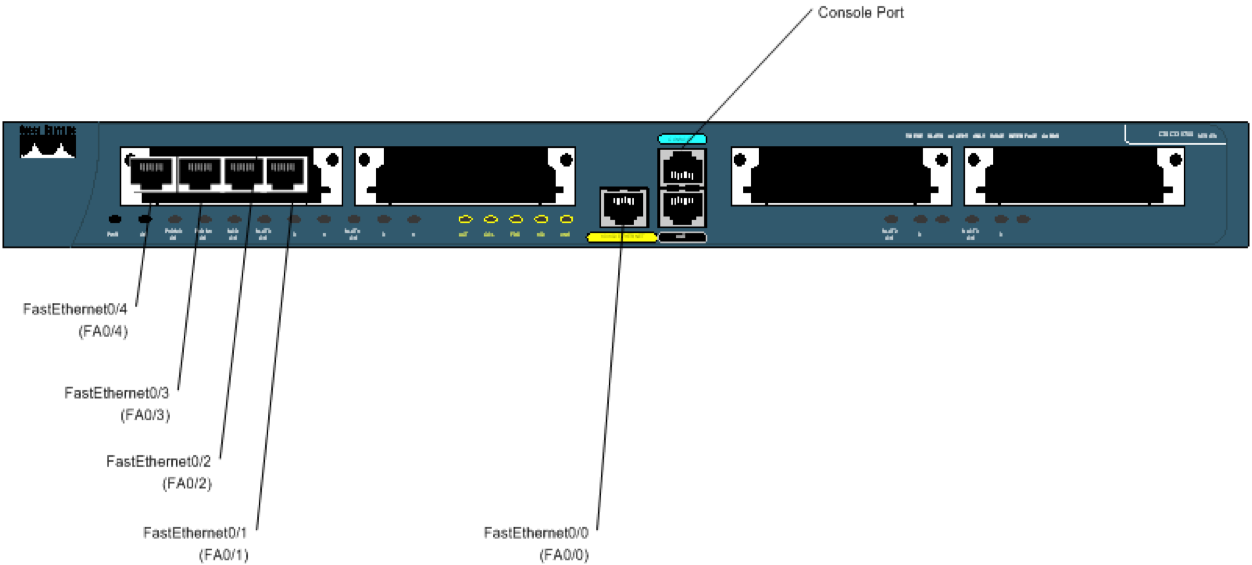
\includegraphics[width=\columnwidth]{graphics/cisco1760.png} 
      \caption{Cisco 1760} \label{fig:cisco1760}
    \end{center}
\end{figure}

The Cisco 1760 router has the following interfaces.
\begin{itemize}
	\item 1 Ethernet Port: FastEthernet0/0
	\item 1 Ethernet Switch Module: vlan1.
\end{itemize}

The 4 ports of the switch module have the following names \iface{FastEthernet0/1}, \iface{FastEthernet0/2}, \iface{FastEthernet0/3}, \iface{FastEthernet0/4}. Note that you can use the shorthand \iface{FA0/X} instead of writing \iface{FastEthernet0/X}.

The easiest way to configure the router is to:
\begin{itemize}
	\item Enable the onboard interface \iface{FA0/0} and give it an IP address.
	\item Turn on one of the ports of the switch module, we recommend you to always use \iface{FA0/1}.
	\item Enable the \iface{Vlan1} interface and assign it an IP address.
	\item We also recommend not changing any of the VLAN settings on the switch module.
\end{itemize}

In IOS this becomes:

\begin{cmdblock}
	Router1(config)# interface FastEthernet0/1
	Router1(config-if)# no shutdown
	Router1(config-if)# interface vlan1
	Router1(config-if)# ip address 10.0.2.1 255.255.255.0
	Router1(config-if)# no shutdown
\end{cmdblock}

Figure~\ref{fig:cisco-internal} shows a logical representation of the internal operation of the Cisco1760, and how the virtual interface \iface{Vlan1} can be configured with an IP address.

\begin{figure}[h!t]
    \begin{center}  
      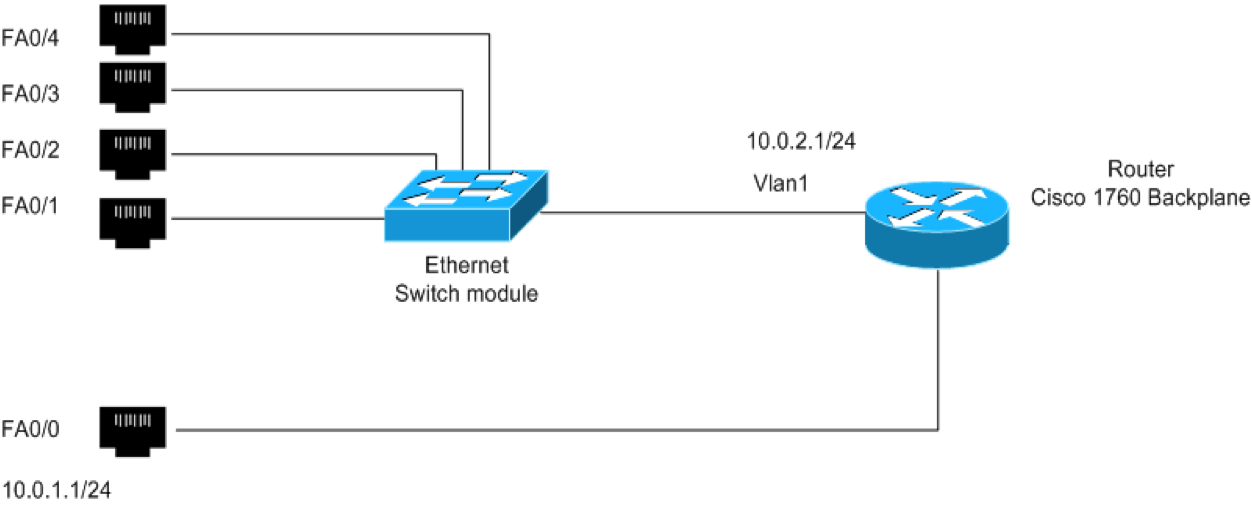
\includegraphics[width=\columnwidth]{graphics/cisco-internal.png} 
      \caption{Cisco 1760 Switch Module} \label{fig:cisco-internal}
    \end{center}
\end{figure}

The following exercises use basic commands from the Cisco IOS that are needed to configure a Cisco router.
\begin{enumerate}
	\item Start a minicom session on PC1 which is connected to Router1 with a serial cable.
	\item Configure Router1 with the IP addresses given in Table \ref{tab:lab3-network1}.
		\begin{cmdblock}
	Router1> enable
	Password: <enable secret>
	Router1# configure terminal
	Router1(config)# no ip routing
	Router1(config)# ip routing
	Router1(config)# interface FastEthernet0/0 
	Router1(config-if)# ip address 10.0.2.1 255.255.255.0 
	Router1(config-if)# no shutdown
	Router1(config-if)# interface FastEthernet0/1
	Router1(config-if)# no shutdown
	Router1(config-if)# interface vlan1
	Router1(config-if)# ip address 10.0.3.1 255.255.255.0 
	Router1(config-if)# no shutdown
	Router1(config-if)# end
		\end{cmdblock}
	\item When you are done, use the following command to check the changes you made to the router configuration, and save the output:
		\begin{cmdblock}
	Router1# show interfaces 
	Router1# show running-config
		\end{cmdblock}
	\item Analyze the output to ensure that you have configured the router correctly.
\end{enumerate}

\begin{questions}
	\q{2.C.1}{Include the output from Step 3 in your lab report.}
\end{questions}
	
	
\subsubsection{Exercise 2-d. Setting static routing table entries on a Cisco router}

Next you must add static routes to the routing table of Router1. The routing table must be configured so that it conforms to the network topology shown in Figure \ref{fig:lab3-network1} and Table \ref{tab:lab3-network1}.

The IOS command to configure static routing is \cmd{ip route}. The command can be used to show, clear, add or delete entries in the routing table. Below is a summary of the commands.

\boxinfo{The following can be executed in the privileged EXEC mode.:
	\begin{description}
		\item[\texttt{show ip route}]\hfill \\
			Display the contents of the routing table.
		\item[\texttt{clear ip route *}]\hfill \\
			Delete all routing table entries.
		\item[\texttt{show ip cache}]\hfill \\
			Display the routing cache.
	\end{description}
}

\boxinfo{The following can can be executed in the Global Configuration mode.
	\begin{description}
		\item[\texttt{ip route-cache}]\hfill \\
			Enable route caching. By default, route caching is enabled on a router.
		\item[\texttt{no ip route-cache}]\hfill \\
			Disable route caching.
		\item[\texttt{ip route destination mask gw\_address}]\hfill \\
			Add a static routing table entry to destination with netmask \cmd{mask}. The argument \cmd{gw\_address} is the IP address of the next hop router.
		\item[\texttt{ip route destination mask Iface}]\hfill \\
			Add a static routing table entry to destination with netmask \cmd{mask}. Here, the next hop information is the name of a network interface (e.g., \iface{FastEthernet0/0}).
		\item[\texttt{no ip route destination mask gw\_address no ip route destination mask Iface}]\hfill \\
			Delete the route table entry with \cmd{destination}, \cmd{mask}, and \cmd{gw\_address} or \cmd{Iface} from the routing table.
	\end{description}
}

We next show some examples for adding and deleting routing table entries in IOS. Compare these commands to the corresponding Linux commands in Part 2, Exercise 1-c. As in Linux, whenever an IP address is configured for a network interface, routing table entries for the directly connected network are added automatically.

The command for adding a route for the network prefix 10.21.0.0/16 with 10.11.1.4 as the next hop address is
\begin{cmdblock}
	Router1(config)#ip route 10.21.0.0 255.255.0.0 10.11.1.4 
\end{cmdblock}

The command to add a host route to IP address 10.0.2.31 with the next hop set to 10.0.1.21 is
\begin{cmdblock}
	Router1(config)#ip route 10.0.2.31 255.255.255.255 10.0.1.21
\end{cmdblock}

In IOS,a host route is identified by a 32-bit prefix. The command to add the IP address 10.0.4.4 as the default gateways is done with the command.
\begin{cmdblock}
     Router1(config) #ip route 0.0.0.0 0.0.0.0 10.0.4.4
\end{cmdblock}

Finally, commands to delete the above entries use the \cmd{no ip route} command.
\begin{cmdblock}
	Router1(config)# no ip route 10.21.0.0 255.255.0.0 10.11.1.4 
	Router1(config)# no ip route 10.0.2.31 255.255.255.255 10.0.1.21 
	Router1(config)# no ip route 0.0.0.0 0.0.0.0 10.0.4.4
\end{cmdblock}

\begin{enumerate}
	\item Display the content of the routing table with \cmd{show ip route}. Note the routing entries that are already present. Save the output.
	\item Add routing entries to Router1, so that the router forwards datagrams for the configuration shown in Figure \ref{fig:lab3-network1}. Routing entries should exist for the following networks:
		\begin{itemize}
			\item 10.0.1.0/24
			\item 10.0.2.0/24
			\item 10.0.3.0/24
		\end{itemize}
	\item Display the routing table again with \cmd{show ip route} and save the output.
\end{enumerate}

\begin{questions}	
	\q{2.D.1}{Include the saved output of the routing table from Step 1 and Step 2. Explain the fields of the routing table entries of the Cisco router. Explain how the routing table has changed from Step 1 to Step 3.}
\end{questions}

\newpage
\subsection{Finalizing and Exploring the Router Configuration}
If the configuration of PC2 and Router1 was done correctly, it is now possible to send IP datagrams between any two machines in the network shown in Figure \ref{fig:lab3-network1}. However, if the network is not configured properly, you need to debug and test your setup. The table below illustrates several common problems that may arise. Since it is impossible to cover all scenarios, network debugging is a crucial skill that you need to obtain for your lab experiments to work well.

\begin{table}[h!t]
	\centering
	\begin{tabular}{ | p{4cm} | p{4cm} | p{4cm} | }
		\hline
		\textbf{Problem} & \textbf{Possible Causes} &  \textbf{Debugging} \\ \hline
		Traffic does not reach destinations on local network & Network interface not configured correctly.& Verify the interface configuration with \cmd{show protocols} (in IOS) or \cmd{ifconfig} (in Linux) \\
		& & \\
		& Incorrectly connected, faulty, or loose cables. & Most interface cards and Ethernet hubs have green LED status lights. Check if the status lights are on. \\
		& & \\
		& & Verify the connection of the cables.\\
		& & \\
		& & Verify that no cross-over cables are used.\\ \hline
		Traffic reaches router, but is not forwarded to remote networks & IP forwarding is not enabled. & Use \cmd{show protocols} (in IOS) or look into \path{/proc/sys/net/ipv4 /ip\_forward} (in Linux) to display the forwarding status \\
		& & \\
		& Routing tables are not configured correctly. & Display routing tables with \cmd{show ip route} (in IOS) or \cmd{netstat -rn} (in Linux). Run \cmd{traceroute} between all hosts and routers. \\ \hline
		ICMP Request messages reaches destination, but ICMP Reply does not reach source & Routing tables are not correctly configured for the reverse path. & Display routing tables with \cmd{show ip route} (in IOS) or \cmd{netstat -rn} (in Linux). Run \cmd{ping} and \cmd{traceroute} in both directions. \\ \hline
		A change in the routing table has no effect on the flow of traffic. & The ARP cache has old entries. & Delete the ARP cache with \cmd{clear arp} (in IOS) or delete entries with \cmd{arp -d} (in Linux). \\ \hline
	\end{tabular}
\end{table}

\subsubsection*{Exercise 3-A. Finalizing the network setup}

Test the network configuration by issuing ping commands from each host and router to every other host and router. If some ping commands do not work, you need to modify the configuration of routers and hosts. If all ping commands are successful, the network configuration is correct, and you can proceed to the next step.

\subsubsection*{Exercise 3-B. Testing routes with traceroute}

\begin{enumerate}
	\item Start an Wireshark session on PC1.
	\item Execute a \cmd{traceroute} command from PC1 to PC4, and save the output.
		\begin{cmdblock}
	PC1% traceroute 10.0.3.41
		\end{cmdblock}
		Observe how \cmd{traceroute} gathers information on the route.
	\item Stop the traffic capture of Wireshark and save the traffic generated by the \cmd{traceroute} command.
	\item Save the routing table of PC1, PC4, PC2 and Router1.
\end{enumerate}

\begin{questions}
	\q{3.B.1}{Use the Wireshark output and the previously saved routing table to explain the operation of \cmd{traceroute}.}
\end{questions}
	
\subsubsection*{Exercise 3-C. Observe MAC addresses at a router}

When a router forwards an IP datagram from one Ethernet segment to another, it does not modify the IP destination address. However, the destination Ethernet address in the Ethernet header is modified at a router.

This exercise requires manipulations to the ARP cache. The \cmd{arp} command in Linux was covered in Lab 2. Below are the corresponding IOS commands for Cisco routers.

\boxinfo{The following can can be executed in the privileged EXEC mode:
	\begin{description}
		\item[\texttt{ip arp}]\hfill \\
			Display the contents of the ARP cache
		\item[\texttt{clear arp}]\hfill \\
			Delete the entire ARP cache
	\end{description}
}

\boxinfo{The following can can be executed in the Global Configuration mode:
	\begin{description}
	\item[\texttt{arp IPaddress}]\hfill \\
		Add an entry for \cmd{IPaddress} to the ARP cache
	\item[\texttt{no arp IPaddress}]\hfill \\
		Delete the ARP entry for \cmd{IPaddress} from the ARP cache
	\end{description}
}

\begin{enumerate}
	\item Erase all ARP entries on PC1, PC2, PC4 and Router1.
	\item Run Wireshark on both PC1 (interface \iface{eth0}) and PC4 (interface \iface{eth0}).
	\item Issue a \cmd{ping} command on PC1 to PC4.
		\begin{cmdblock}
	PC1% ping -c 5 10.0.3.41
		\end{cmdblock}
	\item Save the packet transmissions triggered by the \cmd{ping} command, including ARP requests, ARP reply, ICMP echo request, ICMP echo reply on both PC1 and PC4.
\end{enumerate}

\begin{questions}
	\q{3.C.1}{Determine the source and destination addresses in the Ethernet and IP headers, for the ICMP Echo Request messages that were captured at PC1.}
	\q{3.C.2}{Determine the source and destination addresses in the Ethernet and IP headers, for the ICMP Echo Request message that were captured at PC4.}
	\q{3.C.3}{Use your answers above to explain how the source and destination Ethernet and IP addresses are changed when a datagram is forwarded by a router.}
\end{questions}
	
\subsubsection*{Exercise 3-D. Multiple matches in the routing table}

A router or host uses a routing table to determine the next hop of the path of an IP datagram. In Linux, routing table entries are sorted in the order of decreasing prefix length, and are read from top to bottom. In this exercise, you determine how an IP router or Linux PC resolves multiple matching entries in a routing table.

\begin{enumerate}
	\item Add the following routes to the routing table of PC1:
		\begin{cmdblock}
	PC1% route add -net 10.0.0.0 netmask 255.255.0.0 gw 10.0.1.71
	PC1% route add -host 10.0.3.9 gw 10.0.1.81
		\end{cmdblock}
		From Exercise 1-C there should be a network route for the network prefix 10.0.3.0/24. If there is no such route, then add the following entry:
		\begin{cmdblock}
	PC1% route add -net 10.0.3.0 netmask 255.255.255.0 gw 10.0.1.61
		\end{cmdblock}
	\item Referring to the routing table, determine how many matches exist for the following IP addresses:
		\begin{cmdblock}
	10.0.3.9 
	10.0.3.14
	10.0.4.1
		\end{cmdblock}
	\item Start an Wireshark session on PC1, and issue the following ping commands from PC1:
		\begin{cmdblock}
	PC1% ping -c 1 10.0.3.9 
	PC1% ping -c 1 10.0.3.14 
	PC1% ping -c 1 10.0.4.1
		\end{cmdblock}

		Note that gateways with IP addresses 10.0.1.61, 10.0.1.71, and 10.0.1.81 do not exist. However, PC1 still sends ARP Request packets for these IP addresses.
	\item Save the output of Wireshark and PC1's routing table.
\end{enumerate}

\begin{questions}
	\q{3.D}{Use the saved output to indicate the number of matches for each of the IP addresses above. Explain how PC1 resolves multiple matches in the routing table. Only include relevant output data in your report to support your analysis of the data.}
\end{questions}
	
\subsubsection*{Exercise 3-E. Default Routes}
\begin{enumerate}
	\item Delete the routing table entries added in Step 1 of Exercise 3-D above. (Otherwise, the entries interfere with the remaining exercises in this lab.)
	\item Add default routes on PC1 and PC2.
		\begin{itemize}
			\item On PC1, add a default route with PC2 as the default gateway.
			\item On PC2, add a default route with Router1 as the default gateway.
		\end{itemize}
	\item Start to capture traffic on PC1 (on \iface{eth0}) and PC2 (on both \iface{eth0} and \iface{eth1}) with Wireshark.
	\item Issue a \cmd{ping} command from PC1 to a host on a network that does not exist.
		\begin{cmdblock}
	PC1% ping -c 5 10.0.10.110
		\end{cmdblock}
	\item Save the Wireshark output.
\end{enumerate}

\begin{questions}
	\q{3.E.1}{What is the output on PC1, when the ping command is issued?}
	\q{3.E.2}{Determine how far the ICMP Echo Request message travels?}
	\q{3.E.3}{Which ICMP Echo Reply message returns to PC1?}
\end{questions}

\newpage
\subsection{Proxy ARP}
Proxy Address Resolution Protocol (Proxy ARP) is a method by which a router can forward traffic without using its routing table. Proxy ARP is a configuration option, where an IP router responds to ARP Requests that arrive from one of its connected networks for a host that is on another of its connected networks. Without Proxy ARP enabled, an ARP Request for a host on a different network is unsuccessful, since routers do not forward ARP packets to another network.

In this part, you explore how Proxy ARP enables routers to forward an IP datagram even though the sender of the datagram is not aware that the IP datagram should be forwarded to a router. Proxy ARP is enabled and disabled separately on each interface. In IOS, proxy ARP is enabled by default.

The commands to enable and disable Proxy ARP in the IOS Interface configuration mode are:
\begin{cmdblock}
	ip proxy-arp
	no ip proxy-arp
\end{cmdblock}

\subsubsection*{Exercise 4.}
\begin{enumerate}
	\item Erase the ARP table and the routing table of PC4.
	\item Set the netmask of PC4 to 255.0.0.0, so that PC4 assumes it belongs to network 10.0.0.0/8, instead of belonging to the network 10.0.3.0/24.
	\item Run Wireshark on PC4 (\iface{eth0}), PC2 (\iface{eth1}), and PC1 (\iface{eth0}). Set a display or capture filter to only display ICMP and ARP packets.
	\item Issue a \cmd{ping} from PC4 to PC1:
		\begin{cmdblock}
	PC4% ping -c 2 10.0.1.11
		\end{cmdblock}
		Explore the captured data and interpret the outcome.
		Even though PC4 had no default routing entry in its table for Router1, it was still able to connect to PC1, i.e., you should not observe a ``network unreachable'' error message.
	\item Save the ARP table of PC4 and the packets captured by Wireshark on the hosts.
	\item Explore the captured data and interpret the outcome.
	\item Now, disable Proxy ARP on both interfaces of Router1. Is it still feasible to issue a ping from PC4 to PC1?
	\item Reset the network mask of PC4 to its original value of 255.255.255.0. Then, re-enable Proxy ARP on Router1.
\end{enumerate}

\begin{questions}
	\q{4.1}{Use the captured data to explain the outcome of the exercise. Use the data to explain how Proxy ARP allowed PC4 to communicate with PC1. Include only relevant data from your saved output.}
\end{questions}

\newpage
\subsection{ICMP Route Redirect}
ICMP route redirect messages are sent from a router to a host, when a datagram should have been forwarded to a different router or interface. In Linux, an ICMP Route Redirect message updates the routing cache, but not the routing table.

Both the routing cache and the routing table contain information for forwarding traffic. When a Linux system performs a routing table lookup, it first inspects the routing cache. If no matching entry is found in the cache, Linux performs a lookup in the routing table. After each routing table lookup, an entry is added to the routing cache. The routing cache does not aggregate table entries, and there is a separate entry for each destination IP address. As a consequence, a lookup in the routing cache does not require a longest prefix match. An entry in the routing cache is deleted if it has not been used for some time, usually after 10 minutes. When an ICMP redirect message arrives, an entry is added to the routing cache, but no update is performed to the routing table.

\boxinfo{The following are the commands to display the contents of the routing cache:
	\begin{description}
	\item[\texttt{route -C}]\hfill \\
		In Linux
	\item[\texttt{show ip cache}]\hfill \\
		In IOS
	\end{description}
}

In this part of the lab, you use three Cisco routers. Figure \ref{fig:lab3-network2} and Table \ref{tab:lab3-network2} describe the network configuration for the exercises below.

\begin{figure}[h!t]
	\centering
	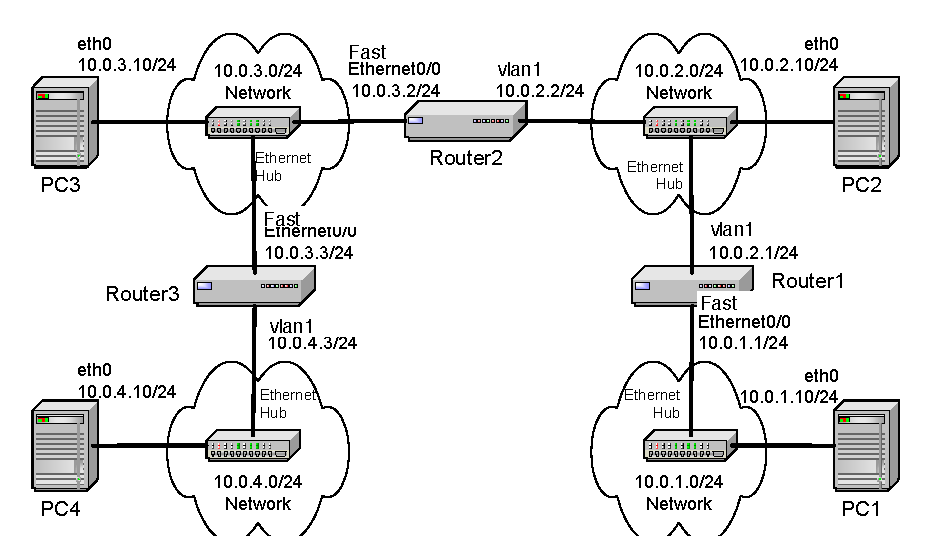
\includegraphics[width=\linewidth]{graphics/lab3-network2-updated.pdf}	
	\caption{Network configuration for Part 5}
	\label{fig:lab3-network2}
\end{figure}

\begin{table}[h!t]
	\centering
	\begin{tabular}{| c | c | c |}	
		\hline
		\textbf{Cisco Router} & \textbf{FastEthernet0/0} & \textbf{vlan1} \\ \hline
		Router1 & 10.0.1.1/24 & 10.0.2.1/24 \\
		Router2 & 10.0.3.2/24 & 10.0.2.2/24 \\
		Router3 & 10.0.3.3/24 & 10.0.4.3/24 \\ \hline
		\textbf{Linux PC} & \textbf{eth0} & \textbf{eth1} \\ \hline
		PC1 & 10.0.1.10/24 & Disabled \\ 
		PC2 & 10.0.2.10/24 & Disabled \\
		PC3 & 10.0.3.10/24 & Disabled \\
		PC4 & 10.0.4.10/24 & Disabled \\ \hline
	\end{tabular}
	\caption{IP addresses for Part 5}
	\label{tab:lab3-network2}
\end{table}

\subsection*{Exercise 5.}
In the network shown in Figure \ref{fig:lab3-network2}, when PC2 sends datagrams with destination 10.0.3.10 (PC3) to 10.0.2.1 (Router1), as opposed to 10.0.2.2 (Router2), then Router1 sends an ICMP Route Redirect message to PC2. The ICMP Route Redirect informs PC2 that it should send datagrams with destination 10.0.3.10 to Router2 instead.

In this exercise, you create the above scenario. First, you will trigger the transmission of an ICMP Route Redirect message and subsequently observe a change to the routing cache.
\begin{enumerate}
	\item Connect the Ethernet interfaces of the routers and the hosts to the hubs as shown in Figure \ref{fig:lab3-network2}.
	\item Delete all routing table entries and all ARP cache entries on all PCs and on Router 1. 
		\begin{itemize}
			\item Delete the routing cache on PC1 with the command:
				\begin{cmdblock}
	PC1% echo "1" > /proc/sys/net/ipv4/route/flush
				\end{cmdblock}
			\item Delete all static routes on Router 1 with the following commands: 
				\begin{cmdblock}
	Router1(config)# no ip routing
	Router1(config)# ip routing
				\end{cmdblock}
			\item Build a new static routing entry on Router1 for network prefix 10.0.3.0/24 as follows:
				\begin{cmdblock}
	Router1(config)# ip route 10.0.3.0 255.255.255.0 10.0.2.2
				\end{cmdblock}
		\end{itemize}
	\item Setup the routing table of PC2 in such a way that it provokes the transmission of an ICMP Route Redirect message as discussed above.
	\item Save the contents of the routing table and the routing cache of Router1, Router2, and PC2.
	\item Use Wireshark to capture the ICMP messages being sent, and issue a ping from PC2 to PC3:
		\begin{cmdblock}
	PC2% ping -c 5 10.0.3.10
		\end{cmdblock}
	\item Save the network traffic and the contents of the routing table and the routing cache after the ICMP Route Redirect messages.
	\item Wait a few minutes and check the contents of the routing cache again. Save the output.
\end{enumerate}

\begin{questions}
	\q{5.1}{Is there a difference between the contents of the routing table and the routing cache immediately after the ICMP Route Redirect message?}
	\q{5.2}{When you viewed the cache a few minutes later, what did you observe?}
	\q{5.3}{Describe how the ICMP Route Redirect works using the output you saved. Include only relevant data from your saved output to support your explanations.}
	\q{5.4}{Explain how Router1, in the above example, knows that datagrams destined to network 10.0.3.10 should be forwarded to 10.0.2.2?}
\end{questions}

\newpage
\subsection{Routing Loops}

A potential problem when setting routing tables manually is that routing loops may occur. In this part of the lab, you intentionally configure a routing loop in the configuration of the routing table and observe what happens to network traffic in such a situation.

\begin{figure}[h!t]
	\centering
	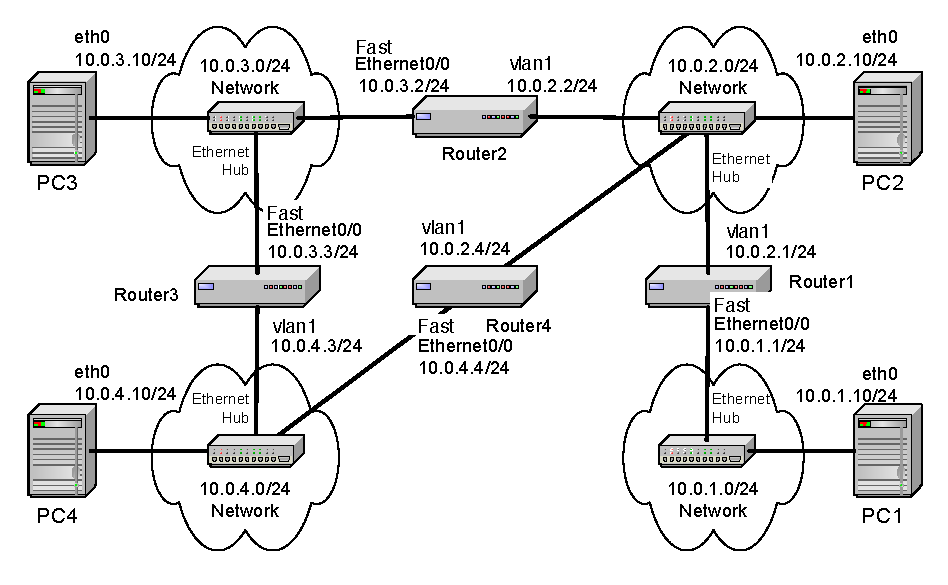
\includegraphics[width=\linewidth]{graphics/lab3-network3-updated.pdf}	
	\caption{Network configuration for Part 6}
	\label{fig:lab3-network3}
\end{figure}

\begin{table}[h!t]
	\centering
	\begin{tabular}{| c | c | c |}	
		\hline
		\textbf{Cisco Router} & \textbf{FastEthernet0/0} & \textbf{vlan1} \\ \hline
		Router4 & 10.0.4.4/24 & 10.0.2.4/24 \\ \hline
	\end{tabular}
	\caption{IP addresses for Part 6}
	\label{tab:lab3-network3}
\end{table}

\subsubsection*{Exercise 6.}
\begin{enumerate}
	\item Add Router4 to the network topology of Part 5 and configure the interfaces as shown in Figure \ref{fig:lab3-network3} and Table \ref{tab:lab3-network3} above.
	\item Configure the routing tables of Router2, Router3 and Router4, so that an ICMP Echo Request message generated by a ping from PC4 to PC1 creates an infinite loop. Issue a \cmd{traceroute} to verify that a loop exists:
		\begin{cmdblock}
	PC4% traceroute 10.0.1.10
		\end{cmdblock}
		You should observe that the traced path is a loop.
	\item Start Wireshark sessions on PC2, PC3, and PC4.
	\item Issue a ping from PC4 to
		\begin{cmdblock}
	PC4% ping -c 1 10.0.1.10
		\end{cmdblock}
		Observe in Wireshark that the same ICMP Echo Request message is looping.
	\item Save the routing tables of Router2, Router3 and Router4. Count the number of times you see the ICMP Echo Request message, as captured by Wireshark on PC4. Save at least two of these ICMP Echo Request messages for the lab report.
\end{enumerate}

\begin{questions}
	\q{6.1}{Are the two ICMP packets that you saved identical? If not, what is different? Include the packet data in your lab report to substantiate your claims.}
	\q{6.2}{Why does the ICMP Echo Request packet not loop forever in the network?}
\end{questions}
	
\newpage	
\subsection{Network Prefixes and Routing}
In this exercise you study the role that network prefixes (netmasks) play when hosts determine if a datagram can be directly delivered or if it must be sent to a router.

This part uses the network setup shown in Figure \ref{fig:lab3-network4}. The network includes one router, four hosts and two hubs. The IP addresses of all devices are given in Table \ref{tab:lab3-network4}. Here, each host has only a default route. In other words, the routing table at a host only knows about the directly connected networks and the default gateway.

\begin{figure}[h!t]
	\centering
	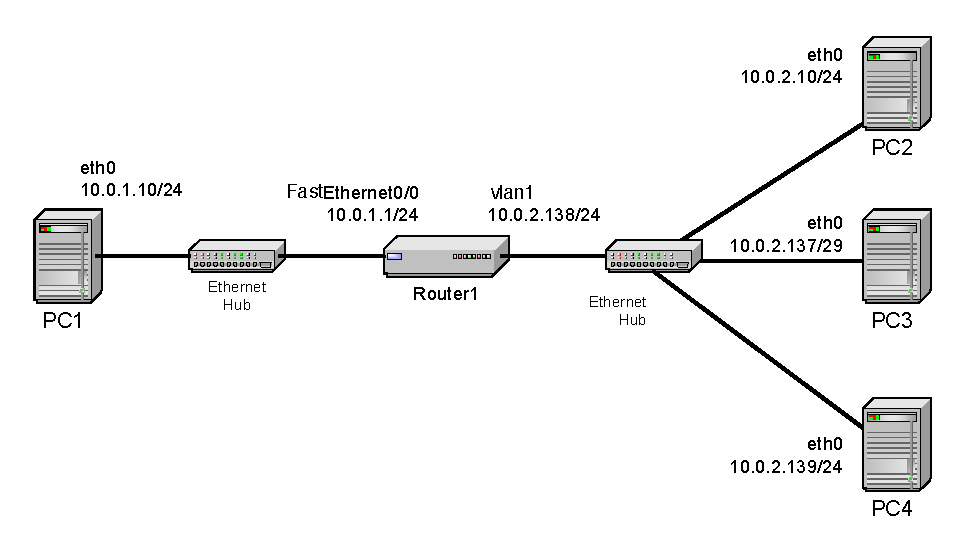
\includegraphics[width=\linewidth]{graphics/lab3-network4-updated.pdf}	
	\caption{Network configuration for Part 7}
	\label{fig:lab3-network4}
\end{figure}

\begin{table}[h!t]
	\centering
	\begin{tabular}{| c | c | c |}	
		\hline
		\textbf{Linux PC} & \textbf{eth0} & \textbf{eth1} \\ \hline
		PC1 & 10.0.1.10/24 & Disabled \\ 
		PC2 & 10.0.2.10/24 & Disabled \\
		PC3 & 10.0.2.137/29 & Disabled \\
		PC4 & 10.0.2.139/24 & Disabled \\ \hline
		\textbf{Cisco Router} & \textbf{FastEthernet0/0} & \textbf{vlan1} \\ \hline
		Router1 & 10.0.1.1/24 & 10.0.2.138/24 \\ \hline
	\end{tabular}
	\caption{IP addresses for Part 7}
	\label{tab:lab3-network4}
\end{table}

\subsubsection{Exercise 7.}
In this exercise, you explore how hosts that are connected to the same local area network, but that have different network addresses or netmasks, communicate or fail to communicate.

\begin{enumerate}
	\item Configure the hosts and the router to conform to the topology shown in Figure \ref{fig:lab3-network4}, using the IP addresses as given in Table \ref{tab:lab3-network4}.
		Note that PC2, PC3, and PC4 have different network addresses and different netmasks.
	\item Add Router1 as default gateway on all hosts. For example, for PC1, the command is:
		\begin{cmdblock}
	PC1% route add default gw 10.0.1.1
		\end{cmdblock}
	\item Issuing ping commands from PC1:
		\begin{enumerate}[label=\alph*.,leftmargin=3em]
			\item Clear the ARP table on all hosts.
			\item Start Wireshark on PC1 and on PC4, and set the capture filter to capture ICMP and ARP packets only.
			\item Check the ARP tables, routing tables and routing caches of each host. Save the output. (Make a note that these are the table entries from Step 3 before the ping is issued.)
			\item Issue a \cmd{ping} command from PC1 to PC2 and PC3 
				\begin{cmdblock}
	PC1% ping -c 2 10.0.2.10
	PC1% ping -c 2 10.0.2.137
				\end{cmdblock}
			\item Save the ARP tables, routing tables and routing caches of each host (Make a note that these are the table entries from Step 3 after the ping is issued.)
			\item Save the output of the ping command at PC1 and the output of Wireshark on PC1 and PC4.
		\end{enumerate}
	\item Issuing a ping command from PC3 to PC4:
		\begin{enumerate}[label=\alph*.,leftmargin=3em]
			\item Clear the ARP table on all hosts.
			\item Start Wireshark on PC3, and set the capture filter to capture ICMP and ARP packets only.
			\item Check the ARP tables, routing tables and routing caches of each host. Save the output. (Make a note that these are the table entries from Step 4 before the ping is issued.)
			\item Issue a \cmd{ping} from PC3 to PC4. 
				\begin{cmdblock}
	PC3% ping -c 3 10.0.2.139
				\end{cmdblock}
			\item Save the ARP tables, routing tables and routing caches of PC3 (Make a note that these are the table entries from Step 4 after the ping is issued.)
			\item Save the output of the \cmd{ping} command and the output of Wireshark on PC3.
		\end{enumerate}
	\item Repeat Step 4, but this time issue a ping from PC3 to PC2. Note that once an entry is made in the routing cache, you cannot repeat the above experiment and obtain the same results; you have to wait until the routing cache is reset (which take some time).
\end{enumerate}

\begin{questions}
	\q{7.1}{Explain what you observed in Steps 3, 4 and 5. Use the saved data to support your answers. Provide explanations of the observations. Try to explain each observed phenomenon, e.g., if you observe more ICMP Echo Requests than ICMP Echo Replies, try to explain the reason.}
	\q{7.2}{If PC3 had no default entry in its table, would you have seen the same results? Explain for each of the pings above what would have been different.}
\end{questions}
